% 4. Experiments & Results
% - [Experimental setup, results, discussion of results incl. their relevancy & limitations; specific organization is very depedenent on the individual situation]
\section{Pretraining}

\subsection{Original Spectrograms}

\begin{figure}[h]
    \centering
    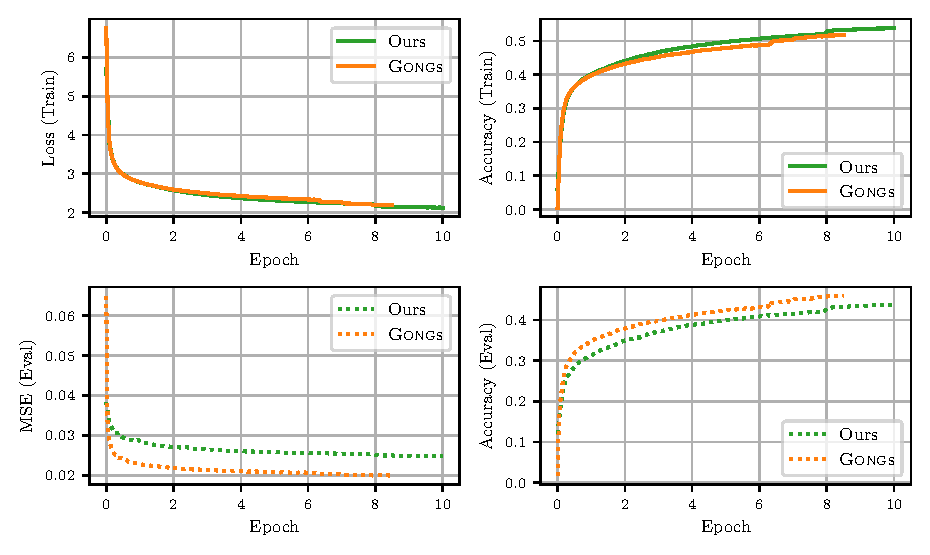
\includegraphics[width=1\linewidth]{img/plots/pretraining_comparison_Gong.pdf}
    \caption{Pretraining result of the model trained on original spectrograms (\gls{mo}).}
    \label{fig:pretrainingResultsOriginalModel}
\end{figure}

Figure \ref{fig:pretrainingResultsOriginalModel} shows the pretraining results of our model trained on original spectrograms (green) compared to the results reported in \cite{gong2022ssast} (orange). The two plots on the top show the performance on the train split, the bottom two plots contain the performance on the test split. The top left plot shows the train loss, calculated using Equation \ref{eq:pretraining-loss}. The bottom left plot shows the \gls{mse} on the test split\footnote{In \cite{gong2022ssast}, they did not keep track of the \gls{infonce} on the evaluation dataset.}. On the right side, we report the accuracy on the train split (top) and the test split (bottom), where accuracy refers to the number of correctly classified patches by the classification head, divided by the total number of masked patches.

As mentioned in \ref{methods_pretraining}, we accidently masked $N=400$ out of $T=499$ patches during evaluation rather than $N=390$, which results in a more challenging task (compared to predicting 400 of 512 patches) and explains the slightly worse performance on the evaluation dataset compared to \cite{gong2022ssast}.

\begin{figure}[h]
    %\begin{adjustwidth}{0cm}{0.0cm}
        \centering
        \begin{tikzpicture}
            \node[anchor=south west,inner sep=0] (image) at (0,0) {
                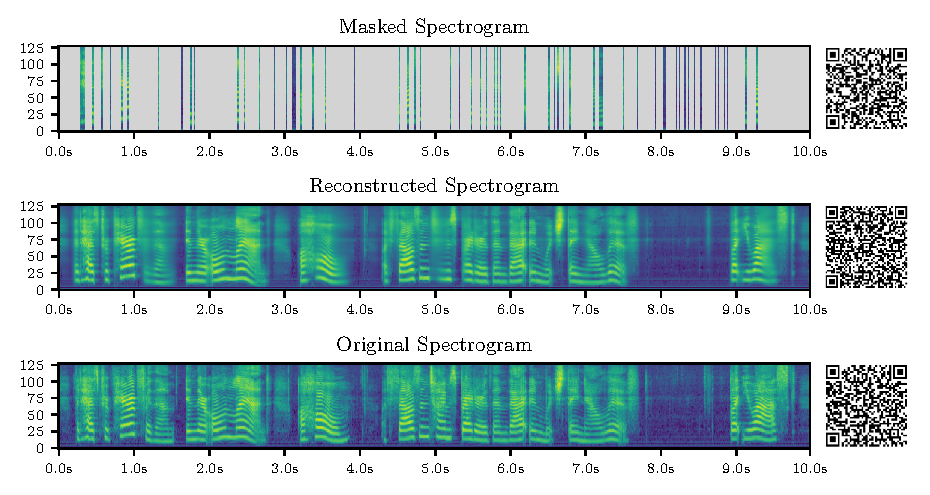
\includegraphics[width=1.0\linewidth]{img/plots/reconstructed_spectrogram_speech_originalModel_with_qr.pdf}
            };
            % Define the scope for the image size
            \begin{scope}[x={(image.south east)},y={(image.north west)}]
                % Define clickable areas
                \node at (0.93,0.18125) {
                    \href{https://github.com/Ironmomo/SpeakerVerificationBA/raw/master/plots_and_audios/audios/original_speech_random_masks_originalModel.wav}{
                        \tikz{\path[fill=none] (0,0) rectangle (0.07,0.165);} % (x, y) ≙ (width, height)
                    }
                };
                \node at (0.93,0.500) {
                    \href{https://github.com/Ironmomo/SpeakerVerificationBA/raw/master/plots_and_audios/audios/reconstructed_speech_random_masks_originalModel.wav}{
                        \tikz{\path[fill=none] (0,0) rectangle (0.07,0.165);}
                    }
                };
                \node at (0.93,0.81875) {
                    \href{https://github.com/Ironmomo/SpeakerVerificationBA/raw/master/plots_and_audios/audios/masked_speech_random_masks_originalModel.wav}{
                        \tikz{\path[fill=none] (0,0) rectangle (0.07,0.165);}
                    }
                };
            \end{scope}
        \end{tikzpicture}
        \caption{Spectrogram with randomly sampled mask indices (top), reconstructed spectrogram from the model trained on original spectrograms (middle), original spectrogram (bottom). Resynthesized audio files from each spectrogram can be downloaded by clicking or scanning the corresponding QR-Code.}
        \label{fig:originalModel_spectrogramReconstruction}
    %\end{adjustwidth}
\end{figure}

Figure \ref{fig:originalModel_spectrogramReconstruction} shows the capabilities of the model pretrained on original spectrograms with an example. In the top part of the image, the masked spectrogram is shown. It is masked at $370$ randomly\footnote{A seed of 15 is used for reproducibility.} sampled indices $I$ in the range $\{0, 1, \dots, 498\}$, i.e., $I=\text{RandomSample}(\{0, 1, \dots, 498\},\linebreak 370)$. This corresponds to 7.4 seconds of masked audio. As seen in the middle spectrogram, the reconstruction is very accurate.





%\newpage

% Difference between \newpage, \clearpage, \pagebreak:
% \newpage ends the current paragraph, fills the current page with white space and starts a new page.
% \clearpage does something more; it also flushes the float queues, producing pages of floats if necessary, then starts a new page.
% \pagebreak is quite different; tells LaTeX to break the current page at the point of the command. With the optional argument, you can convert the \pagebreak command from a demand to a request. The number must be a number from 0 to 4. The higher the number, the more insistent the request is. This command is useful in the last stage of document production: one can force a page break at a convenient spot for improving the typesetting of the next page. Clearly, the text should be in definitive form for this to be effective.


\subsection{Shuffled Spectrograms}

\begin{figure}[hbt!]
    \centering
    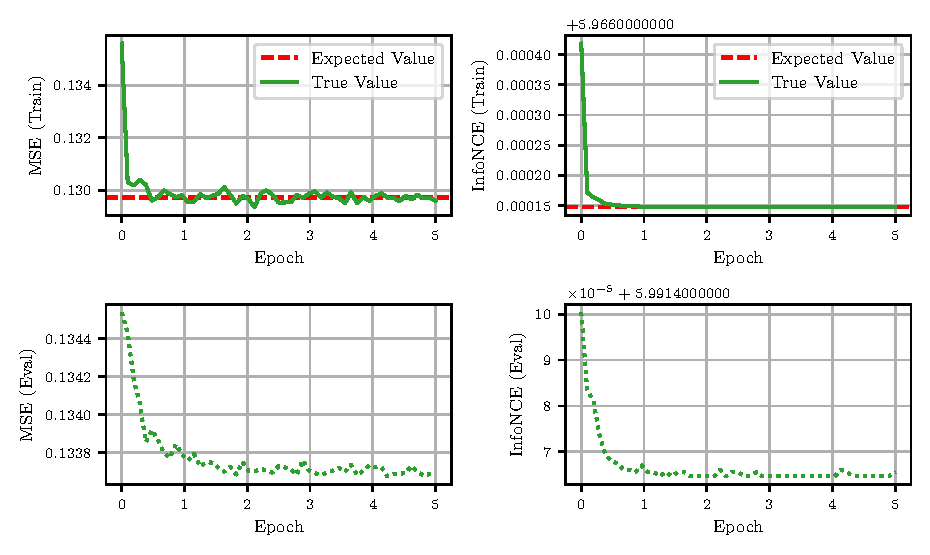
\includegraphics[width=1\linewidth]{img/plots/pretraining_shuffledModel.pdf}
    \caption{Pretraining result of the model trained on shuffled spectrograms (\gls{ms}).}
    \label{fig:pretrainingResultsShuffledModel}
\end{figure}

As seen in Figure \ref{fig:pretrainingResultsShuffledModel}, the loss decreases a bit after the first epoch and then remains more or less at a constant value. The constant value can be calculated for both the \gls{infonce} as well as the \gls{mse} loss. For the train split, this can be done as follows. The procedure for the eval split is analogous.

\begin{algorithm}[hbt!]
\caption{Calculation of Expected \gls{mse} Loss $\mathcal{L}_{g, \text{expected}}$ for the \gls{ms}}
\label{alg:mse_shuffled}
\begin{algorithmic}[1]
\Require{Unlabeled Audio Dataset $\mathcal{D}$, Number of Masked Patches $N$}
\State $\tilde{N}_m = 2N$ \Comment{Number of masked frames}
\State $\tilde{N}_u = L-\tilde{N}_m$ \Comment{Number of unmasked frames}
\State $\texttt{mse\_list} = []$
\For{$X \in \mathcal{D}$}
    \State $I_u=\text{RandomSample}(\{0, 1, \dots, L-1\}, \tilde{N}_u)$ \Comment{Indices of unmasked frames}
    \State $\hat{X} = \frac{1}{\tilde{N}_u} \sum_{i \in I_u} X[i]$ \Comment{Mean vector of unmasked frames}
    \State $I_m = \{0, 1, \ldots, L-1\} \setminus I_u$ \Comment{Indices of masked frames}
    \State $\text{MSE} = \frac{1}{\tilde{N}_m} \sum_{i \in I_m} \text{mean}\left((X[i] - \hat{X})^2\right)$ \Comment{MSE for remaining frames}
    \State Append MSE to $\texttt{mse\_list}$
\EndFor
\State $\mathcal{L}_{g, \text{expected}} = \text{mean}(\texttt{mse\_list})$
\State \textbf{return} $\mathcal{L}_{g, \text{expected}}$
\end{algorithmic}
\end{algorithm}

For the \gls{mse}, the expected loss $\mathcal{L}_{g, \text{expected}}$ can be estimated with Algorithm \ref{alg:mse_shuffled}. The best prediction of a spectrogram with randomly shuffled frames should be to take the average of the unmasked frames as a prediction for the masked ones. To calculate $\mathcal{L}_{g, \text{expected}}$, we can therefore iterate over the dataset, randomly mask $\tilde{N}_m = 2N = 2 \cdot 390 = 780$ frames, calculate the mean in each frequency bin of the remaining $\tilde{N}_u = L-\tilde{N}_m = 998 - 780 = 218$ frames\footnote{The notation $\tilde{N}_m$ and $\tilde{N}_u$ are used to denote the number of masked and unmasked \textit{frames} respectively, to avoid confusion with $N$, which represents the number of masked \textit{patches}.}, and use this as the prediction for the masked frames. Then we calculate the \gls{mse} using Equation \ref{eq:MSE} and take the average over all samples in the dataset, yielding
$$\mathcal{L}_{g, \text{expected}} \approx 0.129726,$$
which seems to be the asymptotic constant{\interfootnotelinepenalty=10000\footnote{To be precise, this value is not exactly the same for each run of Algorithm \ref{alg:mse_shuffled}, since it slightly depends on the (random) selection of the frames used to calculate the average. For a sufficiently large and coherent dataset, this is not a concern.}} the \gls{mse} is approaching.%
%
We can also visualize this property by taking a sample from the dataset, calculating the average of the unmasked frames and plotting a certain number of predicted frames (Figure \ref{fig:average_frame_shuffled_model_predictions}). The predictions are very close to the average of the unmasked frames. This confirms that the model trained on shuffled spectrograms merely learns to calculate the average of the unmasked frames in the spectrogram. The complete masked spectrogram, along with the reconstructed as well as the original spectrogram are shown in Figure \ref{fig:shuffledModel_spectrogramReconstruction}. As can be seen from the middle spectrogram, the reconstruction is very poor, because the model only learned to calculate the average of the unmasked frames in the spectrogram. 

\begin{figure}[hbt!]
    \centering
    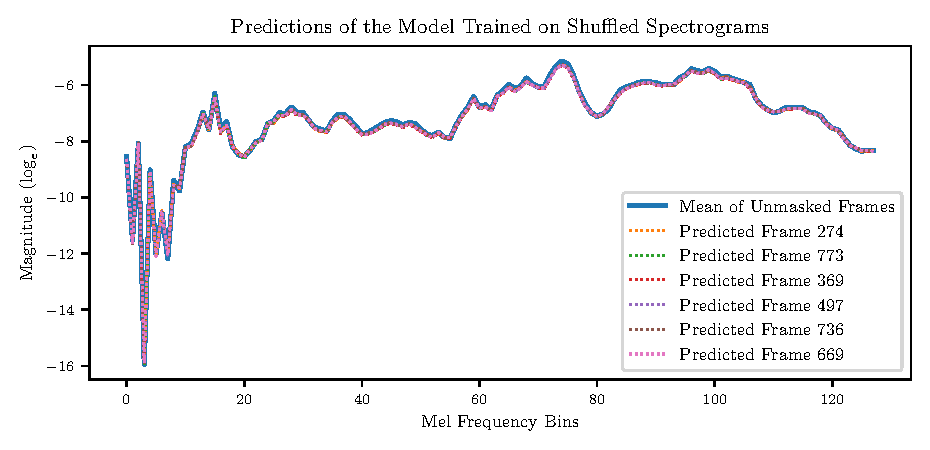
\includegraphics[width=1\linewidth]{img/plots/predictedFrames_shuffled_spectrogram.pdf}
    \caption{Mean of the unmasked frames of the same spectrogram as in Figure~\ref{fig:shuffledModel_spectrogramReconstruction} as well the prediction of the model at six randomly chosen frames from the masked areas.}
    \label{fig:average_frame_shuffled_model_predictions}
\end{figure}

\begin{figure}[hbt!]
    %\begin{adjustwidth}{0cm}{0.0cm}
        \centering
        \begin{tikzpicture}
            \node[anchor=south west,inner sep=0] (image) at (0,0) {
                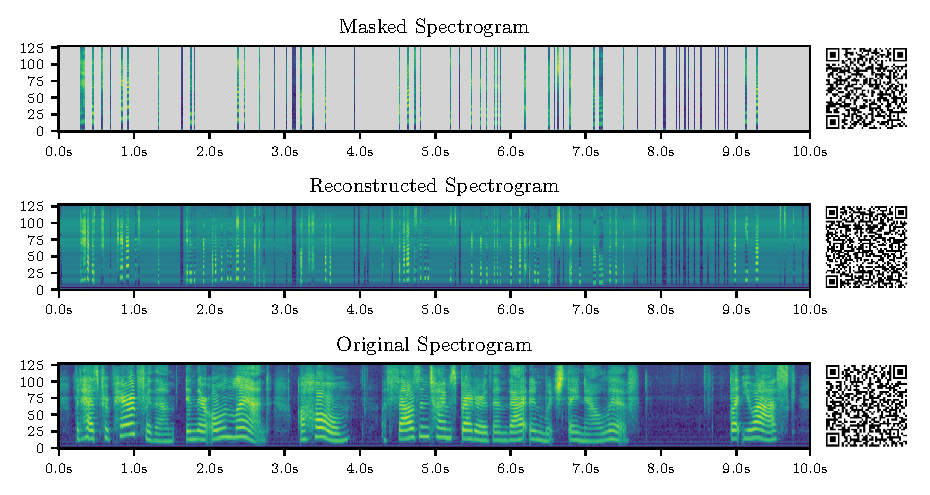
\includegraphics[width=1.0\linewidth]{img/plots/reconstructed_spectrogram_speech_shuffledModel_with_qr.pdf}
            };
            % Define the scope for the image size
            \begin{scope}[x={(image.south east)},y={(image.north west)}]
                % Define clickable areas
                \node at (0.93,0.18125) {
                    \href{https://github.com/Ironmomo/SpeakerVerificationBA/raw/master/plots_and_audios/audios/original_speech_random_masks_shuffledModel.wav}{
                        \tikz{\path[fill=none] (0,0) rectangle (0.07,0.165);} % (x, y) ≙ (width, height)
                    }
                };
                \node at (0.93,0.500) {
                    \href{https://github.com/Ironmomo/SpeakerVerificationBA/raw/master/plots_and_audios/audios/reconstructed_speech_random_masks_shuffledModel.wav}{
                        \tikz{\path[fill=none] (0,0) rectangle (0.07,0.165);}
                    }
                };
                \node at (0.93,0.81875) {
                    \href{https://github.com/Ironmomo/SpeakerVerificationBA/raw/master/plots_and_audios/audios/masked_speech_random_masks_shuffledModel.wav}{
                        \tikz{\path[fill=none] (0,0) rectangle (0.07,0.165);}
                    }
                };
            \end{scope}
        \end{tikzpicture}
        \caption{Spectrogram with randomly sampled mask indices (top), reconstructed spectrogram from the model trained on shuffled spectrograms (middle), original spectrogram (bottom). Resynthesized audio files from each spectrogram can be downloaded by clicking or scanning the corresponding QR-Code.}
        \label{fig:shuffledModel_spectrogramReconstruction}
    %\end{adjustwidth}
\end{figure}

For the \gls{infonce}, each masked frame has an equal probability of being the correct one at any given location. This scenario occurs if 
\begin{equation}
\label{eq:condition_for_equal_prob_infonce}
\frac{\exp(c_i * x_i)}{\sum_{j \in I} \exp(c_i * x_j)} = \frac{1}{N}, \forall i \in I.
\end{equation}

Equation \ref{eq:InfoNCE} can then be simplified as follows:
\begin{equation}
\label{eq:expected_infonce}
\mathcal{L}_{d, \text{expected}} = \frac{-1}{N} \sum_{i \in I} \log_e\left(\frac{1}{N}\right) = \frac{-1}{N} \cdot N \cdot \left(-\log_e(N)\right) = \log_e(N).
\end{equation}

For $N=390$, we obtain
$$\mathcal{L}_{d, \text{expected}} \approx 5.966147,$$
which is exactly the asymptotic value the \gls{infonce} loss approaches, as can be seen in Figure~\ref{fig:pretrainingResultsShuffledModel}. 


\FloatBarrier
\pagebreak [3]
\section{Finetuning}
\label{results_finetuning}

In this section, the results of the finetuning as described in \ref{sec:met:finetuning} are shown and interpreted. This section is structured as follows. First the results of the second finetuning approach (Experiment 2, described in section \ref{methods_finetune_secondAttempt}) using a \gls{mlp} with an output dimension of 256 are discussed. The following sections have been achieved using the first attempt. Exceptions are clearly mentioned. Then the results of the \Gls{eer} are shown and interpreted. Afterwards the results of the cosine similarity are shown and interpreted. The general performance is then evaluated and further interpreted. At the end the results are compared with the \textsc{Neururer} test as described in \ref{foundation_sst}. 

During the last few days before the delivery date of this thesis a 3rd experiment as described in \ref{methods_finetune_thirdAttempt} has been run. The reason for that was because experiment 2 is considered to be a failure. Experiment 3 shows very interesting results leading to another conclusion for this thesis. Due to time concerns the conclusion made from experiment 1 and 2 remains in this thesis. The results of this experiment can be found at the end of this section \ref{results:experiment3}.

\subsection{Experiment 2}

As described in \ref{methods_finetune_secondAttempt}, the second attempt uses a different head to project the (mean pooled) transformer output to speaker embeddings. Due to time limitations only the \gls{ssast} pretrained on the original data, \gls{mo}, has been finetuned, and only on the original data. No further training runs have been done using this head. The model has been trained for 30 epochs. Training it 6x longer than the models trained using approach one (Experiment 1, described in section \ref{methods_finetune_firstAttempt}) should give more insights about the model performance when applying a longer training time. 

\begin{table*}[h]
    \centering
    \caption{Test results of the finetuning using original spectrograms from the Librispeech and Voxceleb 1/2 dataset. \Gls{sr} performance is measured using the \gls{eer}. Bold font indicates best results per model, cell coloring scales with quality per model.}
        \begin{tabular}{>{\centering\arraybackslash}p{1.5cm}| >{\centering\arraybackslash}p{2.5cm} >{\centering\arraybackslash}p{2.5cm}|>{\centering\arraybackslash}p{4cm}  >{\centering\arraybackslash}p{4cm}}
            \hline
            % \multicolumn{2}{c|}{task $\rightarrow$}
            % & \multicolumn{2}{c}{\acrlong{sr}} \\
            \scriptsize{model}
            & \multicolumn{2}{c|}{\scriptsize{pretraining $\downarrow$ / finetuning $\downarrow$ / test $\rightarrow$}}
            & original
            & shuffled \\ 
            \hline
            \gls{moo}
            & original 
            & original
            & \cellcolor[RGB]{255, 155, 0} 13.75
            & \cellcolor[RGB]{235, 215, 0} 11.26 \\
            \hline
        \end{tabular}
    \label{finetuning_v2_results_transformer}
\end{table*}

\begin{table*}[h]
    \centering
    \caption{Test results of the finetuning using original spectrograms from the Librispeech and Voxceleb 1/2 dataset. \Gls{sr} performance is measured using the cosine similarity for positive pairs and for negative pairs.}
        \begin{tabular}{>{\centering\arraybackslash}p{1.5cm}| >{\centering\arraybackslash}p{2.5cm} >{\centering\arraybackslash}p{2.5cm}|>{\centering\arraybackslash}p{4cm}  >{\centering\arraybackslash}p{4cm}}
            \hline
            % \multicolumn{2}{c|}{task $\rightarrow$}
            % & \multicolumn{2}{c}{\acrlong{sr}} \\
            \scriptsize{model}
            & \multicolumn{2}{c|}{\scriptsize{pretraining $\downarrow$ / finetuning $\downarrow$ / test $\rightarrow$}}
            & original
            & shuffled \\ 
            \hline
            \gls{moo}
            & original 
            & original
            & \cellcolor[RGB]{255, 255, 255} Pos.: 0.979 Neg.: 0.723
            & \cellcolor[RGB]{255, 255, 255} Pos.: 0.927 Neg.: 0.717 \\
            \hline
        \end{tabular}
    \label{finetuning_v2_similarity_transformer}
\end{table*}

The \gls{eer} is shown in table \ref{finetuning_v2_results_transformer}. The performance has decreased. The reasons for that cannot be fully explained. One supposition is that the embedding dimension is too small. To underline this presumption, further research would need to be done. It is suggested to apply different optimizer or hyperparameter to minimize the risk of converting to a local minimum.

When evaluating the cosine similarity in Table \ref{finetuning_v2_similarity_transformer}, the cosine similarity for positive pairs approaches the optimal value of 1. However, the cosine similarity for negative pairs, which ideally should be near 0, is relatively high. This discrepancy indicates suboptimal performance.


\subsection{Experiment 1}

The results of experiment 1 are shown in table \ref{finetuning_v1_results_transformer}. While not being state-of-the-art, they are within the same order of magnitude as the models tested in \cite{neururer2023deep} (Table \ref{sst_exploitation_results}). Interestingly, \gls{mss} achieves the best performance. \gls{mos} also achieves better performance than \gls{moo} when tested against shuffled spectrograms. This evidence suggests that model performance for \gls{sr} benefits from shuffled spectrograms / achieves better performance when forced to rely solely on \gls{fba}. This hypothesis has been discussed and affirmed in recent research. Shuffling the frames within each block introduces variability in the feature extraction process. This helps the model to generalize better, as it learns to identify speakers based on a more varied set of inputs, rather than being dependent on a specific sequence of frames \cite{barhoush_2021shuffledMFCC}. 

When evaluating the cosine similarity in Table \ref{finetuning_v1_similarity_transformer}, it does not necessarily mean that a high discrepancy between the positive and negative similarities reflect a better EER.

\begin{table*}[h]
    \centering
    \caption{Test results of the finetuning using original and shuffled spectrograms from the Librispeech and Voxceleb 1/2 dataset. \Gls{sr} performance is measured using the \gls{eer}. Bold font indicates best results per model, cell coloring scales with quality per model.}

    \begin{tabular}{>{\centering\arraybackslash}p{1.5cm}| >{\centering\arraybackslash}p{2.5cm} >{\centering\arraybackslash}p{2.5cm}|>{\centering\arraybackslash}p{4cm}  >{\centering\arraybackslash}p{4cm}}
        \hline
        \scriptsize{model}
        & \multicolumn{2}{c|}{\scriptsize{pretraining $\downarrow$ / finetuning $\downarrow$ / test $\rightarrow$}} & original & shuffled \\
        \hline
        \gls{moo}
        & \multirow{2}{*}{original} 
        & original
        & \cellcolor[RGB]{85, 255, 0} 10.63
        & \cellcolor[RGB]{255, 215, 0} 12.13 \\
        \gls{mos}
        & 
        & shuffled
        & \cellcolor[RGB]{255, 39, 0} 15.61
        & \cellcolor[RGB]{65, 255, 0} \textbf{10.47} \\
        \hdashline
        \gls{mso}
        & \multirow{2}{*}{shuffled} & original
        & \cellcolor[RGB]{245, 235, 0} 11.87
        & \cellcolor[RGB]{245, 255, 0} 11.69\\
        \gls{mss}
        & 
        & shuffled
        & \cellcolor[RGB]{0, 255, 0} 8.41
        & \cellcolor[RGB]{0, 255, 0} \textbf{7.84}\\
        \hline
    \end{tabular}

    \label{finetuning_v1_results_transformer}
\end{table*}


\begin{table*}[h]
    \centering
    \caption{Test results of the finetuning using original and shuffled spectrograms from the Librispeech and Voxceleb 1/2 dataset. \Gls{sr} performance is measured using the cosine similarity for positive pairs and for negative pairs.}

    \begin{tabular}{>{\centering\arraybackslash}p{1.5cm}| >{\centering\arraybackslash}p{2.5cm} >{\centering\arraybackslash}p{2.5cm}|>{\centering\arraybackslash}p{4cm}  >{\centering\arraybackslash}p{4cm}}
        \hline
        \scriptsize{model}
        & \multicolumn{2}{c|}{\scriptsize{pretraining $\downarrow$ / finetuning $\downarrow$ / test $\rightarrow$}} & original & shuffled \\
        \hline
        \gls{moo}
        & \multirow{2}{*}{original} 
        & original
        & \cellcolor[RGB]{255, 255, 255} Pos.: 0.913 Neg.: 0.163
        & \cellcolor[RGB]{255, 255, 255} Pos.: 0.798 Neg.: 0.167 \\
        \gls{mos}
        & 
        & shuffled
        & \cellcolor[RGB]{255, 255, 255} Pos.: 0.918 Neg.: 0.526
        & \cellcolor[RGB]{255, 255, 255} Pos.: 0.864 Neg.: 0.105 \\
        \hdashline
        \gls{mso}
        & \multirow{2}{*}{shuffled} & original
        & \cellcolor[RGB]{255, 255, 255} Pos.: 0.786 Neg.: 0.238
        & \cellcolor[RGB]{255, 255, 255} Pos.: 0.81 Neg.: 0.148 \\
        \gls{mss}
        & 
        & shuffled
        & \cellcolor[RGB]{255, 255, 255} Pos.: 0.809 Neg.: 0.418
        & \cellcolor[RGB]{255, 255, 255} Pos.: 0.767 Neg.: 0.326 \\
        \hline
    \end{tabular}

    \label{finetuning_v1_similarity_transformer}
\end{table*}

% for powerpoint

% \clearpage
% \newpage

% \begin{table*}[h]
%     \centering
%     \caption*{EER in \%, using \textbf{\underline{two}} MLPs as a finetuning head.}
%         \begin{tabular}{>{\centering\arraybackslash}p{2.5cm} >{\centering\arraybackslash}p{2.5cm}|>{\centering\arraybackslash}p{4cm}  >{\centering\arraybackslash}p{4cm}}
%             \hline
%             % \multicolumn{2}{c|}{task $\rightarrow$}
%             % & \multicolumn{2}{c}{\acrlong{sr}} \\
%             \multicolumn{2}{c|}{\scriptsize{pretraining $\downarrow$ / finetuning $\downarrow$ / test $\rightarrow$}}
%             & original
%             & shuffled \\ 
%             \hline
%             original & original
%             & \cellcolor[RGB]{255, 155, 0} 13.75 
%             & \cellcolor[RGB]{255, 215, 0} 12.13 \\
%             \hline
%         \end{tabular}
%     \label{pp1}
% \end{table*}


% \begin{table*}[h]
%     \centering
%     \caption*{EER in \%, using \textbf{\underline{one}} MLP as a finetuning head.}

%     \begin{tabular}{>{\centering\arraybackslash}p{2.5cm} >{\centering\arraybackslash}p{2.5cm}|>{\centering\arraybackslash}p{4cm}  >{\centering\arraybackslash}p{4cm}}
%         \hline
%         % \multicolumn{2}{c|}{task $\rightarrow$} & \multicolumn{2}{c}{\acrlong{sr}} \\
%         \multicolumn{2}{c|}{\scriptsize{pretraining $\downarrow$ / finetuning $\downarrow$ / test $\rightarrow$}} & original & shuffled \\
%         \hline
%         \multirow{2}{*}{original} & original
%         & \cellcolor[RGB]{85, 255, 0} 10.63 
%         & \cellcolor[RGB]{255, 215, 0} 12.13 \\
%         & shuffled
%         & \cellcolor[RGB]{255, 39, 0} 15.61 
%         & \cellcolor[RGB]{65, 255, 0} \textbf{10.47} \\
%         \hdashline
%         \multirow{2}{*}{shuffled} & original
%         & \cellcolor[RGB]{245, 235, 0} 11.87 
%         & \cellcolor[RGB]{245, 255, 0} 11.69 \\
%         & shuffled
%         & \cellcolor[RGB]{0, 255, 0} 8.41
%         & \cellcolor[RGB]{0, 255, 0} \textbf{7.84} \\
%         \hline
%     \end{tabular}
%     \label{pp2}
% \end{table*}

% end 


\subsection{Neururer Test}


Comparing the obtained \glspl{eer} with the results reported in \cite{neururer2023deep} reveals a similar pattern. The performance of \gls{mos} and \gls{mss} relative to \gls{moo} and \gls{mso} does not result in a deterioration of \gls{sr} performance; rather, an improvement in \gls{sr} performance is observed. Consequently, this thesis provides evidence that transformers do not possess a significant inductive bias that makes them more reliant on \gls{sst} compared to other architectures.



\subsection{General Evaluation}

The findings of this thesis provide evidence that transformer networks do not inherently possess an inductive bias to learn \gls{sst}. However, this does not refute the hypothesis that transformer networks can be directed to learn \gls{sst}, thereby achieving more robust performance in \gls{sr}.

\subsubsection{Model Improvements}
\label{result}

We postulate that the performance of the \gls{ssast} for \gls{sr} can be enhanced, potentially yielding results that support the thesis of an inductive bias to learn \gls{sst}. To improve performance, we recommend increasing the batch size and extending the training duration. Additionally, exploring various hyperparameters should be considered.

Research indicates that contrastive learning benefits from larger batch sizes \cite{changyou_2022BatchSize}. Increased batch sizes in contrastive learning facilitate better exploration of the data space, resulting in more diverse negative samples and more accurate gradient estimates.

Figure \ref{fig:loss:finetune} illustrates the train and test loss over five epochs during fine-tuning of \gls{mo} on original spectrograms, producing \gls{moo}. Based on these loss functions, we assumed that a minimum in the loss landscape had been reached, rendering five epochs sufficient. However, consultations with Prof. Dr. Thilo Stadelmann, our supervisor, suggest that this assumption may be incorrect. Phenomena such as \textit{grokking} can lead to improvements in generalization well beyond the point of overfitting \cite{power2022grokking}.

\begin{figure}[hbt!]
    \centering
    \begin{tikzpicture}
    \settowidth{\imagewidth}{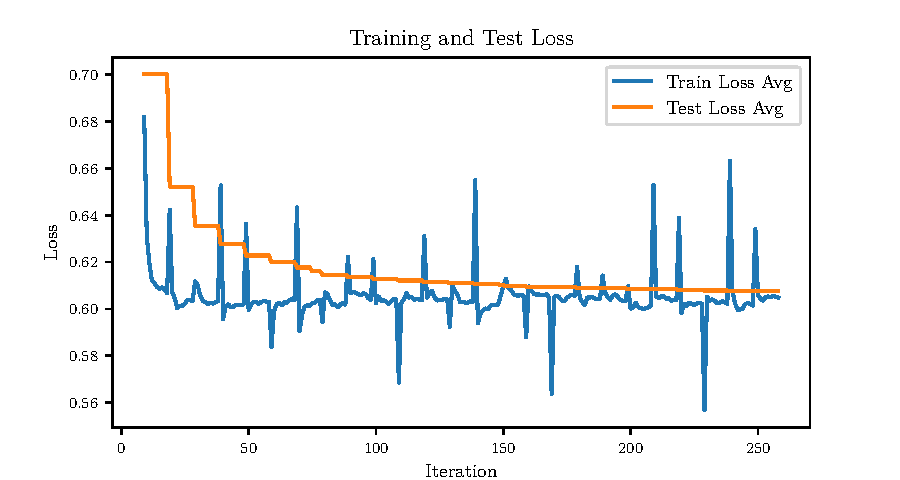
\includegraphics{img/plots/eer_finetuned_model_batch128.pdf}}
    \settoheight{\imageheight}{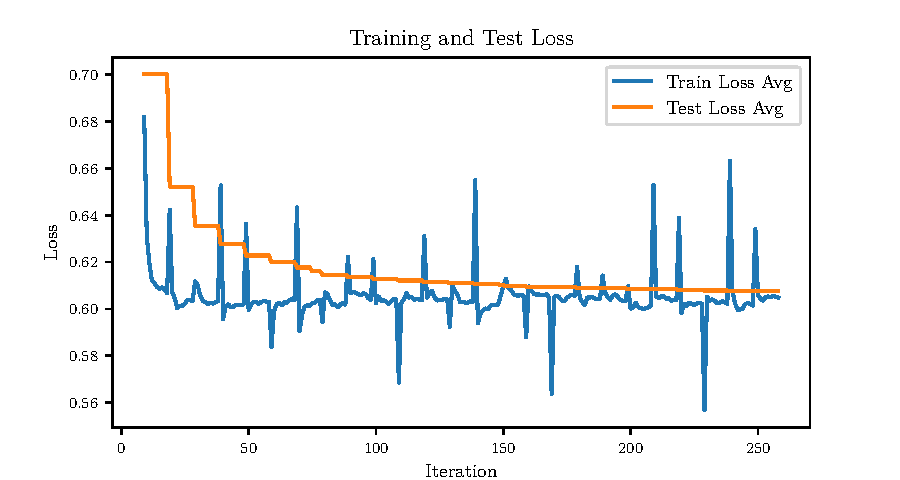
\includegraphics{img/plots/eer_finetuned_model_batch128.pdf}}
        \node[anchor=south west,inner sep=0] (image) at (0,0) {
            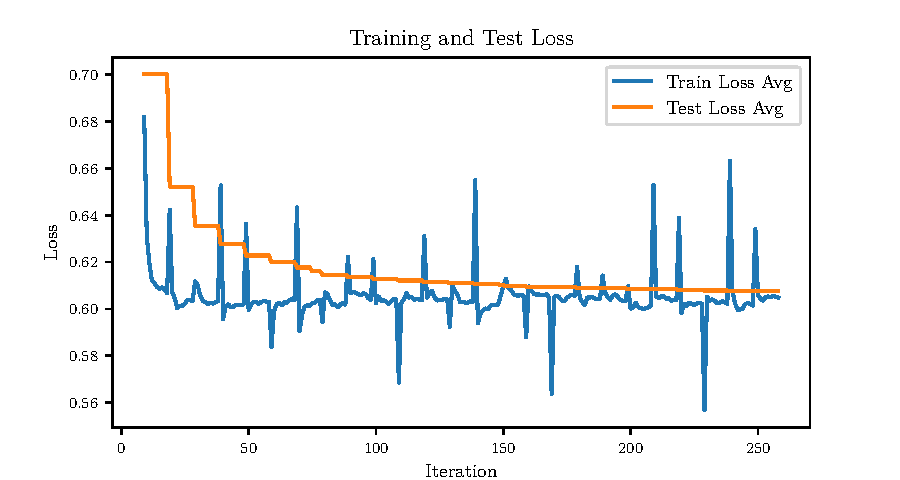
\includegraphics[width=1\linewidth, clip, viewport=0 0.0\imageheight{} \imagewidth{} 0.89\imageheight{}]{img/plots/eer_finetuned_model_batch128.pdf}
        };
    %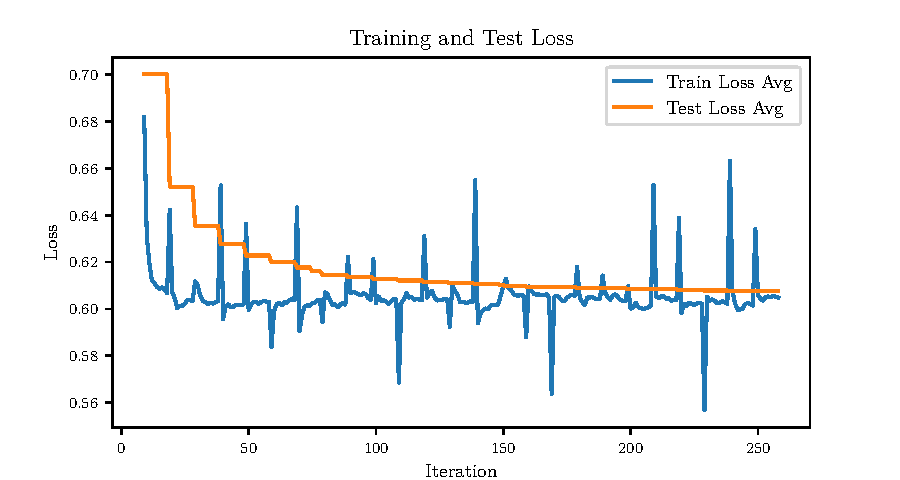
\includegraphics[width=1\linewidth]{img/plots/eer_finetuned_model_batch128.pdf}
    \end{tikzpicture}
    \caption{Training and test loss of \gls{moo} during 5 epochs.}
    \label{fig:loss:finetune}
\end{figure}


\subsection{Experiment 3}
\label{results:experiment3}

As delineated in \ref{methods_finetune_thirdAttempt}, a third experimental iteration has been conducted over the past few days preceding the submission of this thesis. The results derived from this experiment may provide additional substantiation for the hypothesis articulated in \ref{result}, specifically that transformer networks indeed possess an inductive bias towards learning \gls{sst}. Table \ref{finetuning_v3_results_transformer} corroborates that extended training duration enhances performance for \gls{sr}, yielding optimal outcomes. Additionally, the observed performance decline between original and shuffled spectrograms is significantly more pronounced than in previous results.

When evaluating the cosine similarity in table \ref{finetuning_v3_similarity_transformer}, a significant discrepancy between the positive and negative similarities indicates an improved \gls{eer}. However, the poor performance on the shuffled data is evidenced by cosine similarity values that are very close to each other.

\subsubsection{Validity of Neururer's Hypothesis}

To ascertain the validity of Neururer's hypothesis, it is imperative to train an additional model using shuffled spectrograms and assess its performance. Should it be demonstrated that a model trained on shuffled spectrograms fails to surpass the performance of the current model, this would constitute definitive evidence that transformer networks harbor an inductive bias for learning \gls{sst}. However, within the scope of this thesis, the results presented in tables \ref{finetuning_v2_results_transformer} and \ref{finetuning_v3_results_transformer} are not directly comparable.


\begin{table*}[h]
    \centering
    \caption{Test results of the finetuning using original spectrograms from the Librispeech and Voxceleb 1/2 dataset. \Gls{sr} performance is measured using the \gls{eer}. Bold font indicates best results per model, cell coloring scales with quality per model.}
        \begin{tabular}{>{\centering\arraybackslash}p{1.5cm}| >{\centering\arraybackslash}p{2.5cm} >{\centering\arraybackslash}p{2.5cm}|>{\centering\arraybackslash}p{4cm}  >{\centering\arraybackslash}p{4cm}}
            \hline
            % \multicolumn{2}{c|}{task $\rightarrow$}
            % & \multicolumn{2}{c}{\acrlong{sr}} \\
            \scriptsize{model}
            & \multicolumn{2}{c|}{\scriptsize{pretraining $\downarrow$ / finetuning $\downarrow$ / test $\rightarrow$}}
            & original
            & shuffled \\ 
            \hline
            \gls{moo}
            & original 
            & original
            & \cellcolor[RGB]{0, 255, 0} \textbf{6.54}
            & \cellcolor[RGB]{255, 0, 0} 19.61 \\
            \hline
        \end{tabular}
    \label{finetuning_v3_results_transformer}
\end{table*}


\begin{table*}[h]
    \centering
    \caption{Test results of the finetuning using original spectrograms from the Librispeech and Voxceleb 1/2 dataset. \Gls{sr} performance is measured using the cosine similarity for positive pairs and for negative pairs.}
        \begin{tabular}{>{\centering\arraybackslash}p{1.5cm}| >{\centering\arraybackslash}p{2.5cm} >{\centering\arraybackslash}p{2.5cm}|>{\centering\arraybackslash}p{4cm}  >{\centering\arraybackslash}p{4cm}}
            \hline
            % \multicolumn{2}{c|}{task $\rightarrow$}
            % & \multicolumn{2}{c}{\acrlong{sr}} \\
            \scriptsize{model}
            & \multicolumn{2}{c|}{\scriptsize{pretraining $\downarrow$ / finetuning $\downarrow$ / test $\rightarrow$}}
            & original
            & shuffled \\ 
            \hline
            \gls{moo}
            & original 
            & original
            & \cellcolor[RGB]{255, 255, 255} Pos.: 0.929 Neg.: 0.425
            & \cellcolor[RGB]{255, 255, 255} Pos.: 0.972 Neg.: 0.913 \\
            \hline
        \end{tabular}
    \label{finetuning_v3_similarity_transformer}
\end{table*}